\section{Exemplos de comandos}

\subsection{Margens}

A norma ABNT NBR 6022:2018 não estabelece uma margem específica a ser utilizada
no artigo científico. Dessa maneira, caso deseje alterar as margens, utilize os
comandos abaixo:

\begin{verbatim}
   \setlrmarginsandblock{3cm}{3cm}{*}
   \setulmarginsandblock{3cm}{3cm}{*}
   \checkandfixthelayout
\end{verbatim}

\subsection{Duas colunas}

É comum que artigos científicos sejam escritos em duas colunas. Para isso,
adicione a opção \texttt{twocolumn} à classe do documento, como no exemplo:

\begin{verbatim}
   \documentclass[article,11pt,oneside,a4paper,twocolumn]{abntex2}
\end{verbatim}

É possível indicar pontos do texto que se deseja manter em apenas uma coluna,
geralmente o título e os resumos. Os resumos em única coluna em documentos com
a opção \texttt{twocolumn} devem ser escritos no ambiente
\texttt{resumoumacoluna}:

\begin{verbatim}
   \twocolumn[              % INICIO DE ARTIGO EM DUAS COLUNAS

     \maketitle             % pagina de titulo

     \renewcommand{\resumoname}{Nome do resumo}
     \begin{resumoumacoluna}
        Texto do resumo.
      
        \vspace{\onelineskip}
 
        \noindent
        \textbf{Palavras-chave}: latex. abntex. editoração de texto.
     \end{resumoumacoluna}
   
   ]                        % FIM DE ARTIGO EM DUAS COLUNAS
\end{verbatim}

\subsection{Recuo do ambiente \texttt{citacao}}

Na produção de artigos (opção \texttt{article}), pode ser útil alterar o recuo
do ambiente \texttt{citacao}. Nesse caso, utilize o comando:

\begin{verbatim}
   \setlength{\ABNTEXcitacaorecuo}{1.8cm}
\end{verbatim}

Quando um documento é produzido com a opção \texttt{twocolumn}, a classe
\textsf{abntex2} automaticamente altera o recuo padrão de 4 cm, definido pela
ABNT NBR 10520:2002 seção 5.3, para 1.8 cm.

\section{Cabeçalhos e rodapés customizados}

Diferentes estilos de cabeçalhos e rodapés podem ser criados usando os
recursos padrões do \textsf{memoir}.

Um estilo próprio de cabeçalhos e rodapés pode ser diferente para páginas pares
e ímpares. Observe que a diferenciação entre páginas pares e ímpares só é
utilizada se a opção \texttt{twoside} da classe \textsf{abntex2} for utilizado.
Caso contrário, apenas o cabeçalho padrão da página par (\emph{even}) é usado.

Veja o exemplo abaixo cria um estilo chamado \texttt{meuestilo}. O código deve
ser inserido no preâmbulo do documento.

\begin{verbatim}
%%criar um novo estilo de cabeçalhos e rodapés
\makepagestyle{meuestilo}
  %%cabeçalhos
  \makeevenhead{meuestilo} %%pagina par
     {topo par à esquerda}
     {centro \thepage}
     {direita}
  \makeoddhead{meuestilo} %%pagina ímpar ou com oneside
     {topo ímpar/oneside à esquerda}
     {centro\thepage}
     {direita}
  \makeheadrule{meuestilo}{\textwidth}{\normalrulethickness} %linha
  %% rodapé
  \makeevenfoot{meuestilo}
     {rodapé par à esquerda} %%pagina par
     {centro \thepage}
     {direita} 
  \makeoddfoot{meuestilo} %%pagina ímpar ou com oneside
     {rodapé ímpar/onside à esquerda}
     {centro \thepage}
     {direita}
\end{verbatim}

Para usar o estilo criado, use o comando abaixo imediatamente após um dos
comandos de divisão do documento. Por exemplo:

\begin{verbatim}
   \begin{document}
     %%usar o estilo criado na primeira página do artigo:
     \pretextual
     \pagestyle{meuestilo}
     
     \maketitle
     ...
     
     %%usar o estilo criado nas páginas textuais
     \textual
     \pagestyle{meuestilo}
     
     \chapter{Novo capítulo}
     ...
   \end{document}  
\end{verbatim}

Outras informações sobre cabeçalhos e rodapés estão disponíveis na seção 7.3 do
manual do \textsf{memoir} \cite{memoir}.

\section{Inserindo figuras no texto}
\label{sec:imag}

Há algumas formas de inserir uma figura num texto em latex, nesta secção será salientado algumas, e na secção \ref{sec:rgrap}, você poderá verificar como inserir gráficos do R em um texto em latex.

Figuras podem ser criadas diretamente em latex,como o exemplo da \autoref{fig_circulo}.

\begin{figure}[htb]
   \caption{\label{fig_circulo}A delimitação do espaço}
   \begin{center}
      \setlength{\unitlength}{5cm}
      \begin{picture}(1,1)
         \put(0,0){\line(0,1){1}}
         \put(0,0){\line(1,0){1}}
         \put(0,0){\line(1,1){1}}
         \put(0,0){\line(1,2){.5}}
         \put(0,0){\line(1,3){.3333}}
         \put(0,0){\line(1,4){.25}}
         \put(0,0){\line(1,5){.2}}
         \put(0,0){\line(1,6){.1667}}
         \put(0,0){\line(2,1){1}}
         \put(0,0){\line(2,3){.6667}}
         \put(0,0){\line(2,5){.4}}
         \put(0,0){\line(3,1){1}}
         \put(0,0){\line(3,2){1}}
         \put(0,0){\line(3,4){.75}}
         \put(0,0){\line(3,5){.6}}
         \put(0,0){\line(4,1){1}}
         \put(0,0){\line(4,3){1}}
         \put(0,0){\line(4,5){.8}}
         \put(0,0){\line(5,1){1}}
         \put(0,0){\line(5,2){1}}
         \put(0,0){\line(5,3){1}}
         \put(0,0){\line(5,4){1}}
         \put(0,0){\line(5,6){.8333}}
         \put(0,0){\line(6,1){1}}
         \put(0,0){\line(6,5){1}}
      \end{picture}
   \end{center}
   \legend{Fonte: os autores}
\end{figure}

Ou então figuras podem ser incorporadas de arquivos externos, como é o caso da \autoref{fig_grafico}. Se a figura que for incluída se tratar de um diagrama, um gráfico ou uma ilustração que você mesmo produza, priorize o uso de imagens vetoriais no formato PDF. Com isso, o tamanho do arquivo final do trabalho será menor, e as imagens terão uma apresentação melhor, principalmente quando impressas, uma vez que imagens vetorias são perfeitamente escaláveis para qualquer dimensão. Nesse caso, se for utilizar o Microsoft Excel para produzir gráficos, ou o Microsoft Word para produzir ilustrações, exporte-os como PDF e os incorpore ao documento conforme o exemplo abaixo. No entanto, para manter a coerência no uso de software livre (já que você está usando \LaTeX e \abnTeX), teste a ferramenta \textsf{InkScape}\index{InkScape} (\url{http://inkscape.org/}). Ela é uma excelente opção de código-livre para produzir ilustrações vetoriais, similar ao CorelDraw\index{CorelDraw} ou ao Adobe Illustrator\index{Adobe Illustrator}. De todo modo, caso não seja possível utilizar arquivos de imagens como PDF, utilize qualquer outro formato, como JPEG, GIF, BMP, etc. Nesse caso, você pode tentar aprimorar as imagens incorporadas com o software livre \textsf{Gimp}\index{Gimp} (\url{http://www.gimp.org/}). Ele é uma alternativa livre ao Adobe Photoshop\index{Adobe Photoshop}.


\begin{figure}[htb]
   \caption{\label{fig_grafico}Gráfico produzido em Excel e salvo como PDF}
   \begin{center}
      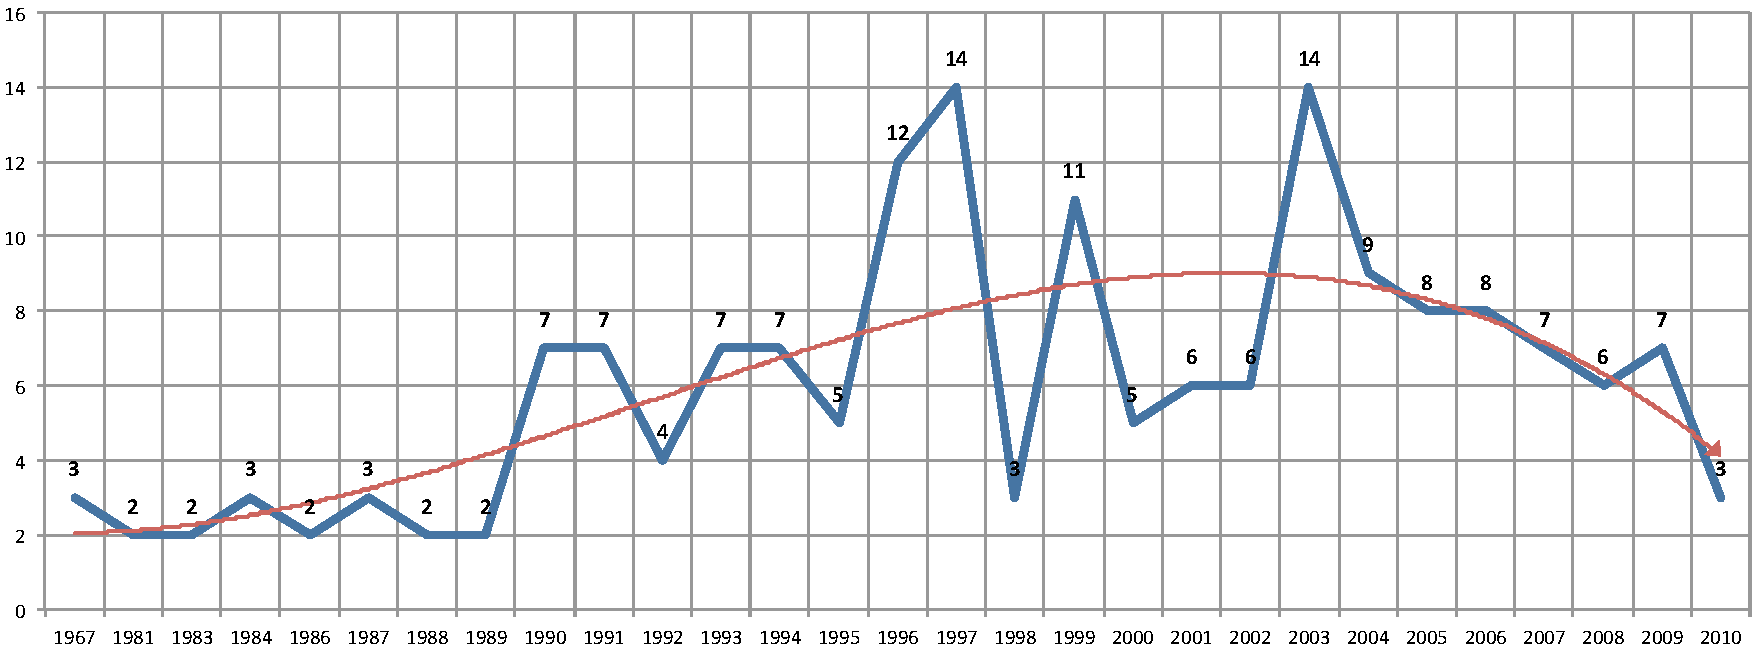
\includegraphics[scale=0.5]{img-grafico.pdf}
   \end{center}
   \legend{Fonte: \citeonline[p. 24]{araujo2012}}
\end{figure}

% ---
\subsection{Figuras em \emph{minipages}}
% ---

\emph{Minipages} são usadas para inserir textos ou outros elementos em quadros com tamanhos e posições controladas. Veja o exemplo da \autoref{fig_minipage_imagem1} e da \autoref{fig_minipage_grafico2}.

\begin{figure}[htb]
   \label{teste}
   \centering
   \begin{minipage}{0.4\textwidth}
      \centering
      \caption{Imagem 1 da minipage} \label{fig_minipage_imagem1}
      
\includegraphics[scale=0.9]{img-marca.pdf}
      \legend{Fonte: Produzido pelos autores}
   \end{minipage}
   \hfill
   \begin{minipage}{0.4\textwidth}
      \centering
      \caption{Grafico 2 da minipage} \label{fig_minipage_grafico2}
      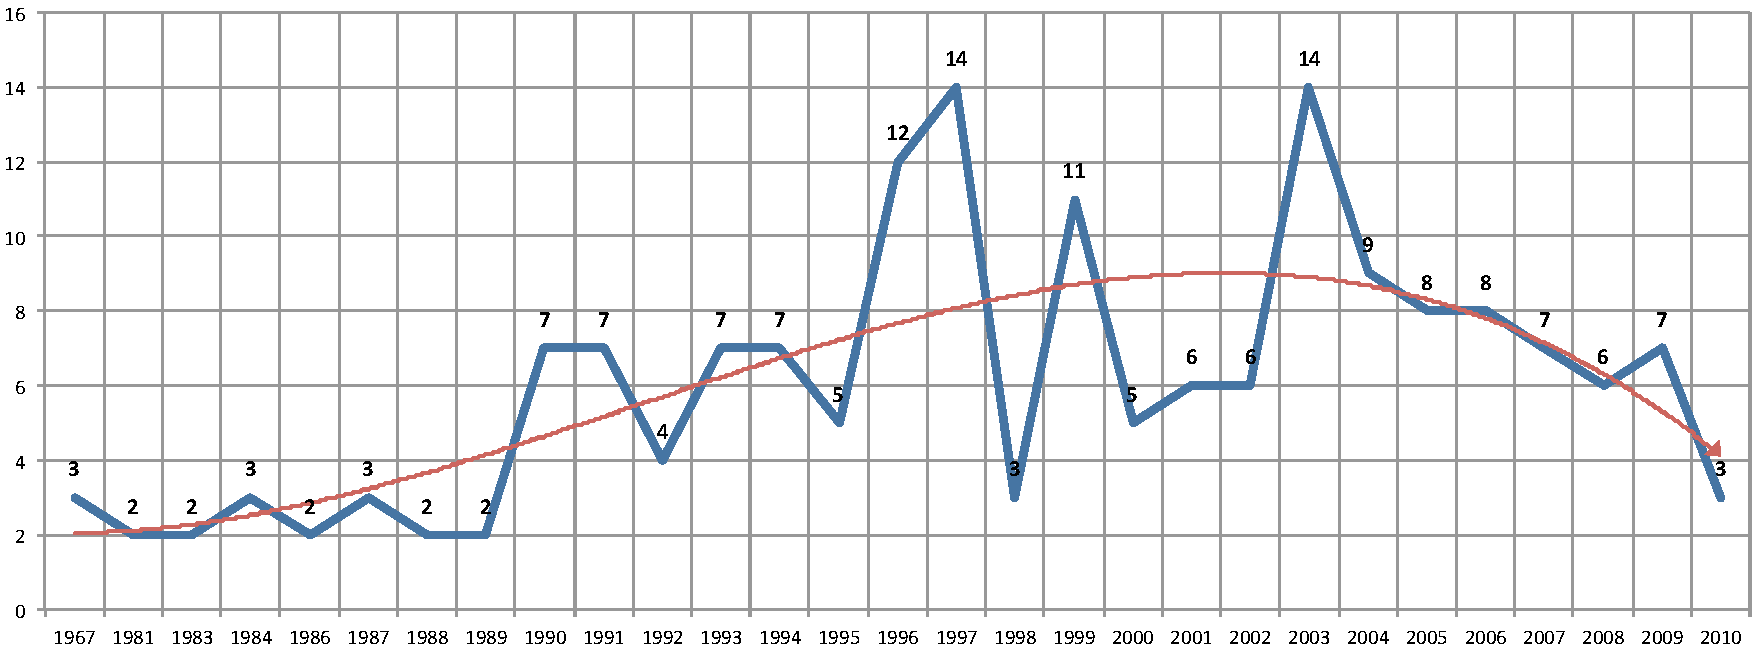
\includegraphics[scale=0.2]{img-grafico.pdf}
      \legend{Fonte: \citeonline[p. 24]{araujo2012}}
   \end{minipage}
\end{figure}

Observe que, segundo a \citeonline[seções 4.2.1.10 e 5.8]{NBR14724:2011}, as ilustrações devem sempre ter numeração contínua e única em todo o documento:

\begin{citacao}
   Qualquer que seja o tipo de ilustração, sua identificação aparece na parte superior, precedida da palavra designativa (desenho, esquema, fluxograma, fotografia, gráfico, mapa, organograma, planta, quadro, retrato, figura, imagem, entre outros), seguida de seu número de ordem de ocorrência no texto, em algarismos arábicos, travessão e do respectivo título. Após a ilustração, na parte inferior, indicar a fonte consultada (elemento obrigatório, mesmo que seja produção do próprio autor), legenda, notas e outras informações necessárias à sua compreensão (se houver). A ilustração deve ser citada no texto e inserida o mais próximo possível do trecho a que se refere. \cite[seções 5.8]{NBR14724:2011}
\end{citacao}


\subsection{Turtlebot 3}
\label{ss:turtlebot3}
% //todo @alexandre > realizar a implementação da sub-section



